\documentclass[conference]{IEEEtran}

%% INFOCOM addition:
\makeatletter
\def\ps@headings{%
\def\@oddhead{\mbox{}\scriptsize\rightmark \hfil \thepage}%
\def\@evenhead{\scriptsize\thepage \hfil\leftmark\mbox{}}%
\def\@oddfoot{}%
\def\@evenfoot{}}
\makeatother
\pagestyle{headings}

\usepackage[noadjust]{cite}

\usepackage[dvips]{graphicx}

\usepackage{url}

\begin{document}

\title{\texttt{apt-p2p}: A Peer-to-Peer Distributor for Free Software Package Release and Update}
\author{\IEEEauthorblockN{Cameron Dale}
\IEEEauthorblockA{School of Computing Science\\
Simon Fraser University\\
Burnaby, British Columbia, Canada\\
Email: camerond@cs.sfu.ca}
\and
\IEEEauthorblockN{Jiangchuan Liu}
\IEEEauthorblockA{School of Computing Science\\
Simon Fraser University\\
Burnaby, British Columbia, Canada\\
Email: jcliu@cs.sfu.ca}}

\maketitle

\begin{abstract}
A large amount of free software packages are available over the
Internet from many different distributors. Most of these
distributors use the traditional client-server model to handle
requests from users. However, there is an excellent opportunity to
use peer-to-peer techniques to reduce the cost of much of this
distribution, especially due to the altruistic nature of many of
these users. There are no existing solution suitable for this
situation, so we present a new technique for satisfying the needs of
this P2P distribution, which is generally applicable to many of
these distributors' systems. Our method makes use of a DHT for
storing the location of peers, using the cryptographic hash of the
package as a key. To show the simplicity and functionality, we
implement a solution for the distribution of Debian software
packages, including the many DHT customizations needed. Finally, we
analyze our system to determine how it is performing and what effect
it is having.
\end{abstract}

%%%%%%%%%%%%%%%%%%%%%%%%%%%  Section  %%%%%%%%%%%%%%%%%%%%%%%%%%%%

\section{Introduction}
\label{intro}

There are a large number of free software package distributors using
package distribution systems over the Internet to distribute
software to their users. These distributors have developed many
different methods for this distribution, but they almost exclusively
use a client-server model to satisfy user requests. The popularity
and number of users results in a large number of requests, which
usually requires a network of mirrors to handle. Due to the free
nature of this software, many users are willing and able to
contribute upload bandwidth to this distribution, but have no
current way to do this.

We present a new peer-to-peer distribution model to meet these
demands. It is based on many previous implementations of successful
peer-to-peer protocols, especially distributed hash tables (DHT) and
BitTorrent. The model relies on the pre-existence of cryptographic
hashes of the packages, which should uniquely identify it for a
request from other peers. If the peer-to-peer download fails, then
the original request to the server is used as a fallback to prevent
any dissatisfaction from users. The peer can then share this new
package with others through the P2P system.

First, we examine the opportunity that is available for many of
these free software package distributors. We present an overview of
a system that would efficiently satisfy the demands of a large
number of users, and should significantly reduce the currently
substantial bandwidth requirements of hosting this software. We then
present an example implementation based on the Debian package
distribution system. This implementation will be used by a large
number of users, and serves as an example for other free software
distributors of the opportunity that can be met with such a system.

The rest of this paper is organized as follows. The background and motivation are presented in Section~\ref{situation}, and we analyze BitTorrent's use for this purpose in Section~\ref{bittorrent}. We propose
our solution in Section~\ref{opportunity}. We then detail our sample
implementation for Debian-based distributions in Section~\ref{implementation},
including an in-depth look at our DHT
customizations in Section~\ref{custom_dht}. Its performance is evaluated in Section~\ref{analysis}. We examine some related work in Section~\ref{related}, and then
Section~\ref{conclusions} concludes the paper and offers some future directions.

%%%%%%%%%%%%%%%%%%%%%%%%%%%  Section  %%%%%%%%%%%%%%%%%%%%%%%%%%%%

\section{Background and Motivations}
\label{situation}

In the free software society, there are a large number of groups using the Internet to 
collaboratively develop and release their software. The ever increasing power of
modern programming languages and operating systems has made these software, like commercial software, extremely large and complex, which often
consists of many small units (packages). Together with their popularity among users, 
an efficient and reliable management and distribution of these packages over the Internet has become an daunting task. In this section, we offer concrete examples illustrating the 
unique challenges in this context. 

\subsection{Free Software Package Distributor: Examples}
\label{examples}


Most Linux distributions use a software package management system
that fetches packages to be installed from an archive of packages
hosted on a network of mirrors. The Debian project, and other
Debian-based distributions such as Ubuntu and Knoppix, use the
\texttt{apt} (Advanced Package Tool) program, which downloads Debian
packages in the \texttt{.deb} format from one of many HTTP mirrors.
The program will first download index files that contain a listing
of which packages are available, as well as important information
such as their size, location, and a hash of their content. The user
can then select which packages to install or upgrade, and
\texttt{apt} will download and verify them before installing them.

There are also several similar frontends for the RPM-based
distributions. Red Hat's Fedora project uses the \texttt{yum}
program, SUSE uses \texttt{YAST}, while Mandriva has
\texttt{Rpmdrake}, all of which are used to obtain RPMs from
mirrors. Other distributions use tarballs (\texttt{.tar.gz} or
\texttt{.tar.bz2}) to contain their packages. Gentoo's package
manager is called \texttt{portage}, SlackWare Linux uses
\texttt{pkgtools}, and FreeBSD has a suite of command-line tools,
all of which download these tarballs from web servers.

Similar tools have been used for other software packages. CPAN
distributes software packages for the PERL
programming language, using SOAP RPC requests to find and download
files. Cygwin provides many of the
standard Unix/Linux tools in a Windows environment, using a
package management tool that requests packages from websites. There
are two software distribution systems for Mac OSX, fink and
MacPorts, that also retrieve packages in this way.

Direct web downloading is also a common way, often coupled with a hash
verification file to be downloaded next to the desired
file. The hash file usually have the same file name, but with an
added extension identifying the hash used (e.g. \texttt{.md5} for
the MD5 hash). This type of file downloading and verification is
typical of free software hosting facilities that are open to anyone
to use, such as SourceForge.


Given the free nature of these software, there are often a number of users 
motivated by altruism to want to help out with their distribution. 
This is particularly true considering that many of these software are used by
groups that are staffed mostly, or sometimes completely, by
volunteers. They are thus motivated to contribute their network resources, so as to promote the healthy development 
of the volunteer community that released the software. As a matter of fact,
we have see many free mirror sites hosting these software packages for downloading. 
We also naturally expect that peer-to-peer distribution can be implementation in 
this context, which scale well with large user bases and can easily explore the network resources made available by
the volunteers. 



\subsection{Unique Characteristics}
\label{problems}

While it seems straightforward to use an existing peer-to-peer file sharing tool like BitTorrent for
free software package distribution, there are indeed a series of new challenges in this unique scenario:

\subsubsection{Archive Dimensions}

While most of the packages of a software release are very small in
size, there are some that are quite large. There are too many
packages to distribute each individually, but the archive is also
too large to distribute in its entirety. In some archives there are
also divisions of the archive into sections, e.g. by the operating system (OS) or computer
architecture that the package is intended for.

\begin{figure}
\centering
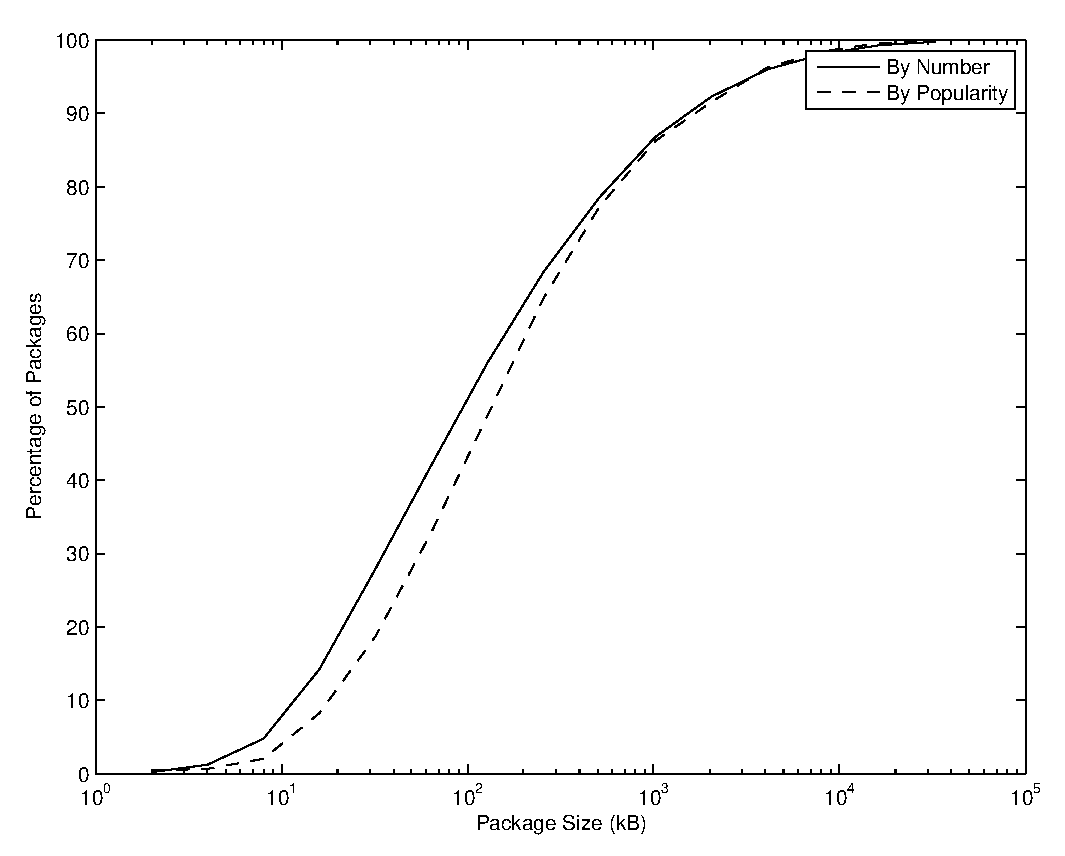
\includegraphics[width=\columnwidth]{apt_p2p_simulation-size_CDF.eps}
\caption{The CDF of the size of packages in a Debian system, both
for the actual size and adjusted size based on the popularity of
the package.}
\label{size_CDF}
\end{figure}

For example, Figure~\ref{size_CDF} shows the size of the packages in the
current Debian distribution. While 80\% of the packages are less than
512~KB, some of the packages are hundreds of megabytes. The entire
archive consists of 22,298 packages and is approximately 119,000 MB
in size. Most of the packages are to be installed in any computer environment, but there are 
also OS- or architecture-specific packages, as shown by the adjusted sizes based on popularity of the packages. ((((more words on how the size is adjusted by popularity))))

\subsubsection{Package Updates}

The software packages being distributed are being constantly
updated. These updates could be the result of the software creators
releasing a new version with improved functionality,
or the distributor updating their packaging of the
software to meet new requirements. Even if the distributor
periodically makes \emph{stable} releases, which are snapshots of
all the packages in the archive at a certain time, updates are still
released for security issues or serious bugs.

\begin{figure}
\centering
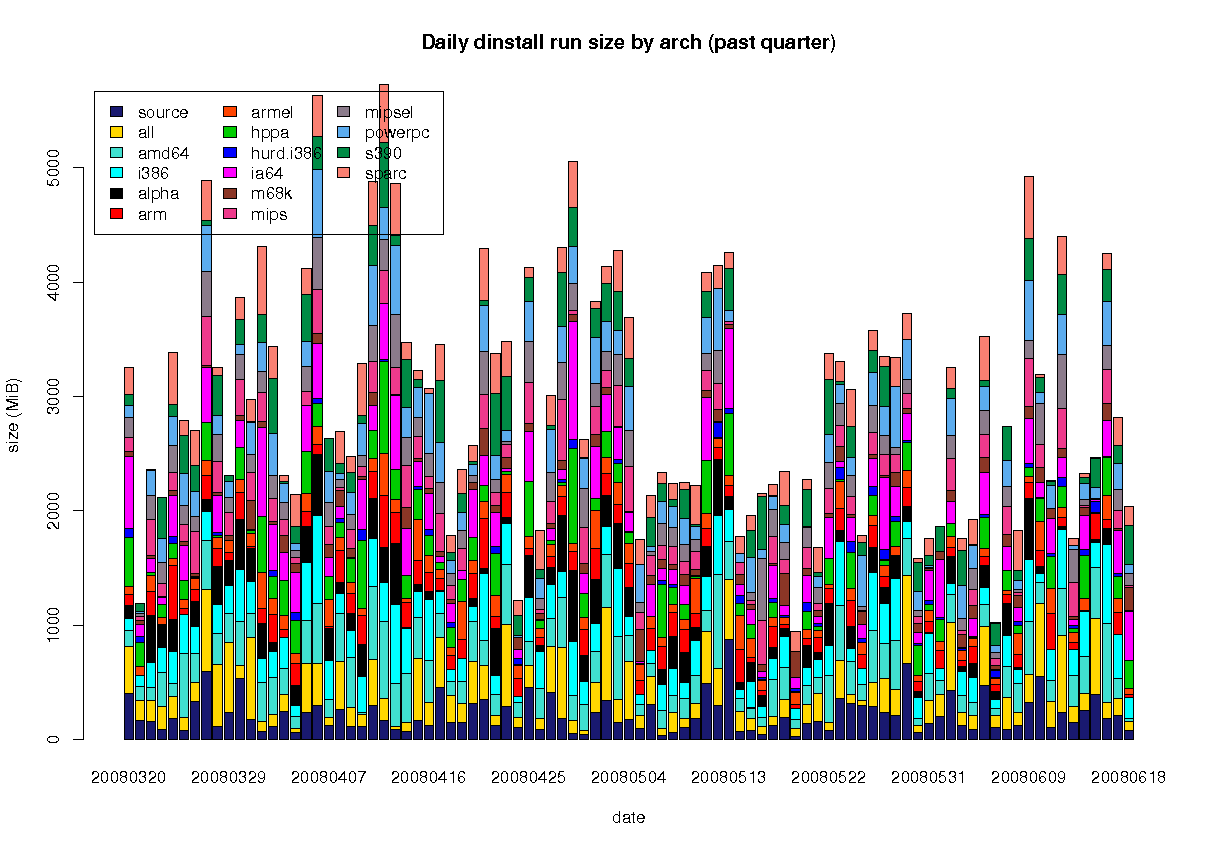
\includegraphics[width=\columnwidth]{size-quarter.eps}
\caption{The amount of data in the Debian archive that is updated
each day, broken down by architecture.}
\label{update_size}
\end{figure}

For example, Figure~\ref{update_size} shows the amount of data in
the Debian archive that was updated each day over a period of 3
months. In every single day, approximately 1.5\% of the 119,000 MB archive is
updated with new versions of packages. Note that this frequency is much higher than
that of most commercial software, mainly because many free software are
developed in a loosely management environment with developers working
asynchronously from worldwide. 

\subsubsection{Limited Interest}

Finally, though there are a large number of packages and a large number of
users, the interest in a particular version of a package can be very 
limited. Specifically, there are core packages that every user has to download, but most
packages would fall in the category of optional or extra, and so are
interesting to only a limited number of people.

\begin{figure}
\centering
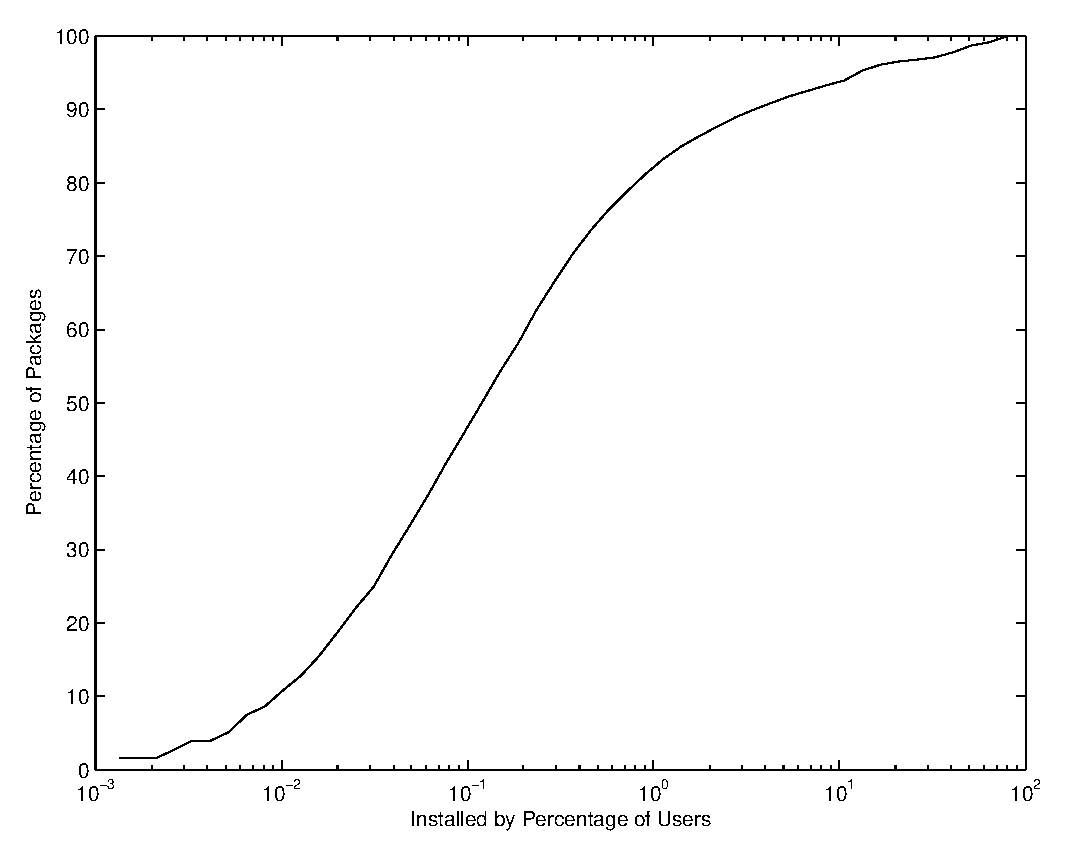
\includegraphics[width=\columnwidth]{apt_p2p_popularity-cdf.eps}
\caption{The CDF of the popularity of packages in a Debian system.}
\label{popularity_CDF}
\end{figure}

For example, the Debian distribution tracks the popularity of its
packages using popcon \cite{popcon}. Figure~\ref{popularity_CDF}
shows the cumulative distribution function of the percentage of all
users who install each package. Though some packages are installed
by everyone, 80\% of the packages are installed by less than 1\% of
users.


%%%%%%%%%%%%%%%%%%%%%%%%%%%  Section  %%%%%%%%%%%%%%%%%%%%%%%%%%%%

\subsection{Why BitTorrent Doesn't Work Well}
\label{bittorrent}

Recently, many distributors make their software available using
BitTorrent \cite{COHEN03}, in particular, for the distribution of CD
images. This straightforward use however is far ineffective, as it requires the
peers to download large numbers of packages that they are not
interested in, and prevents them from updating to new packages
without downloading another image containing a lot of the same
packages they already have. 

An alternative is to create torrents tracking individual packages. Unfortunately, we find that this enhancement can be
quite difficult given the unique characteristic of free software packages. 

First, there is no obvious way to divide the packages into torrents.
Most of the packages are too small, and there are too many packages
in the entire archive to create individual torrents for each one.
On the other hand, all the packages together are too large to track
efficiently as a single torrent. Hence, some division of the archive's
packages into torrents is obviously necessary, but wherever that
split occurs it will cause either some duplication of connections,
or prevent some peers from connecting to others who do have the same
content. In addition, a small number of the packages can be updated every
day which would add new files to the torrent, thereby changing its
\emph{infohash} identifier and making it a new torrent. This will
severely fracture the download population, even though peers in the
new torrent may share 99\% of the packages in common with peers in the
old torrent.

Other issues also prevent BitTorrent from being a good solution to
this problem. In particular, BitTorrent's fixed piece sizes (?KB) that disregard file
boundaries are bigger than many of the packages in the archive. This
will waste peers' downloading bandwidth as they will end up
downloading parts of other packages just to get the piece that
contains the package they do want. 

Finally, note that BitTorrent downloads files
randomly, which does not work well with the interactive package
management tools expectation of sequential downloads. On the other hand, with altruistic peers, incentives to share (upload) 
become a less important issue, and the availability of seeds are not critical, either, as the mirror sites 
can serve in that capacity.



%%%%%%%%%%%%%%%%%%%%%%%%%%%  Section  %%%%%%%%%%%%%%%%%%%%%%%%%%%%

\section{Peer-to-Peer Assisted Distributor: An Overview}
\label{opportunity}

The situation described in Section~\ref{situation} presents a clear
opportunity to use some form of peer-to-peer file-sharing protocol
to allow willing users to contribute upload bandwidth. This sparse
interest in a large number of packages undergoing constant updating
is well suited to the functionality provided by a Distributed Hash
Table (DHT). DHTs require unique keys to store and retrieve strings
of data, for which the cryptographic hashes used by these package
management systems are perfect for. The stored and retrieved strings
can then be pointers to the peers that have the package that hashes
to that key. A downloading peer can lookup the package hash in the
DHT and, if it is found, download the file from those peers and
verify the package with the hash. Once the download is complete, the
peer will add its entry to the DHT indicating that it now has the
package.

The fact that this package is also available to download for free
from a server is very important to our proposal. If the package hash
can not be found in the DHT, the peer can then fallback to
downloading from the original location (i.e. the network of
mirrors). The mirrors thus, with no modification to their
functionality, serve as seeds for the packages in the peer-to-peer
system. Any packages that have just been updated, or that are very
rare, and so don't have any peers available can always be found on
the mirror. Once the peer has completed the download from the mirror
and verified the package, it can then add itself to the DHT as the
first peer for the new package, so that future requests from peers
will not need the mirror.

The trust of the package is also always guaranteed through the use
of the cryptographic hashes. Nothing can be downloaded from a peer
until the hash is looked up in the DHT, so a hash must first come
from a trusted source (i.e. a mirror). Most distributors use index
files that contain hashes for a large number of the packages in
their archive, and which are also hashed. After retrieving the
index's hash from the mirror, the index file can be downloaded from
peers and verified. Then the program has access to all the hashes of
the packages it will be downloading, all of which can be verified
with a \emph{chain of trust} that stretches back to the original
distributor's server.

\subsection{Implementation Options}
\label{imp_options}

There are several ways to implement the desired P2P functionality
into the existing package management software. The functionality can
be directly integrated through modifications to the software, though
this could be difficult as the P2P functionality should be running
at all times. This is needed both for efficient lookups and to
support uploading of already downloaded packages. Unfortunately, the
package management tools typically only run until the download and
install request is complete.

Many of the package management software implementations use HTTP
requests from web servers to download the packages, which makes it
possible to implement the P2P aspect as an almost standard HTTP
caching proxy. This proxy will run as a daemon in the background,
listening for requests from the package management tool for package
files. It will get uncached requests first from the P2P system, or
falling back to the normal HTTP request from a server should it not
be found. For methods that don't use HTTP requests, other types of
proxies may also be possible.

\subsection{Downloading From Peers}
\label{downloading}

Although not necessary, we recommend implementing a download
protocol that is similar to the protocol used to fetch packages from
the distributor's servers. This simplifies the P2P program, as it
can then treat peers and mirrors almost identically when requesting
packages. In fact, the mirrors can be used when there are only a few
slow peers available for a file to help speed up the download
process.

Downloading a file efficiently from a number of peers is where
BitTorrent shines as a peer-to-peer application. Its method of
breaking up larger files into pieces, each with its own hash,
makes it very easy to parallelize the downloading process and
maximize the download speed. For very small packages (i.e. less than
the piece size), this parallel downloading is not necessary, or
even desirable. However, this method should still be used, in
conjunction with the DHT, for the larger packages that are
available.

Since the package management system only stores a hash of the entire
package, and not of pieces of that package, we will need to be able
to store and retrieve these piece hashes using the P2P protocol. In
addition to storing the file download location in the DHT (which
would still be used for small files), a peer will store a
\emph{torrent string} containing the peer's hashes of the pieces of
the larger files. These piece hashes could be compared ahead of time
to determine which peers have the same piece hashes (they all
should), and then used during the download to verify the pieces of
the downloaded package.

%%%%%%%%%%%%%%%%%%%%%%%%%%%  Section  %%%%%%%%%%%%%%%%%%%%%%%%%%%%

\section{\texttt{apt-p2p}: A Practical Implementation}
\label{implementation}

We have created a sample implementation that functions as described
in section \ref{opportunity}, and is freely available for other
distributors to download and modify \cite{apt-p2p}. This software,
called \texttt{apt-p2p}, interacts with the \texttt{apt} tool, which
is found in most Debian-based Linux distributions. \texttt{apt} uses
SHA1 hashes to verify most downloaded files, including the large
index files that contain the hashes of the individual packages. We
chose this distribution system as it is familiar to us, it allows
software contributions, and there are interesting statistics
available for analyzing the popularity of the software packages
\cite{popcon}.

Since all requests from apt are in the form of HTTP downloads from a
server, the implementation takes the form of a caching HTTP proxy.
Making a standard \texttt{apt} implementation use the proxy is then
as simple as prepending the proxy location and port to the front of
the mirror name in \texttt{apt}'s configuration file (i.e.
``localhost:9977/mirrorname.debian.org/\ldots'').

We created a customized DHT based on Khashmir \cite{khashmir}, which
is an implementation of Kademlia \cite{kademlia} using methods
familiar to BitTorrent developers. Khashmir is also the same DHT
implementation used by most of the existing BitTorrent clients to
implement trackerless operation. The communication is all handled by
UDP messages, and RPC (remote procedure call) requests and responses
are all \emph{bencoded} in the same way as BitTorrent's
\texttt{.torrent} files. Khashmir uses the high-level Twisted
event-driven networking engine \cite{twisted}, so we also use
Twisted in our sample implementation for all other networking needs.
More details of this customized DHT can be found below in
Section~\ref{custom_dht}.

Downloading is accomplished by sending simple HTTP requests to the
peers identified by lookups in the DHT to have the desired file.
Requests for a package are made using the package's hash, properly
encoded, as the URL to request from the peer. The HTTP server used
for the proxy also doubles as the server listening for requests for
downloads from other peers. All peers support HTTP/1.1, both in the
server and the client, which allows for pipelining of multiple
requests to a peer, and the requesting of smaller pieces of a large
file using the Range request header.

%%%%%%%%%%%%%%%%%%%%%%%%%%%  Section  %%%%%%%%%%%%%%%%%%%%%%%%%%%%

\section{Customized DHT}
\label{custom_dht}

A large contribution of our work is in the customization and use of
a Distributed Hash Table (DHT). Although our DHT is based on
Kademlia, we have made many improvements to it to make it suitable
for this application. In addition to a novel storage technique to
support piece hashes, we have improved the response time of looking
up queries, allowed the storage of multiple values for each key, and
incorporated some improvements from BitTorrent's tracker-less DHT
implementation.

\subsection{Kademlia Background}
\label{kademlia}

The Kademlia DHT, like most other DHTs, assigns IDs to peers from
the same space that is used for keys. The peers with IDs closest to
the desired key will then store the values for that key. Lookups are
recursive, as nodes are queried in each step that are exponentially
closer to the key than in the previous step.

Nodes in a Kademlia system support four primitive requests.
\texttt{ping} will cause a peer to return nothing, and is only used
to determine if a node is still alive, while \texttt{store} tells a
node to store a value associated with a given key. The most
important primitives are \texttt{find\_node} and
\texttt{find\_value}, which both function recursively to find nodes
close to a key. The queried nodes will return a list of the nodes
they know about that are closest to the key, allowing the querying
node to quickly traverse the DHT to find the nodes close to the
desired key. The only difference between them is that the
\texttt{find\_value} query will cause a node to return a value, if
it has one for that key, instead of a list of nodes.

\subsection{Piece Hash Storage}
\label{pieces}

Hashes of pieces of the larger package files are needed to support
their efficient downloading from multiple peers.
For large files (5 or more pieces), the torrent strings described in
Section~\ref{downloading}
are too long to store with the peer's download info in the DHT. This
is due to the limitation that a single UDP packet should be less
than 1472 bytes to avoid fragmentation.
% For example, for a file of 4 pieces, the peer would need to store a
% value 120 bytes in size (IP address, port, four 20-byte pieces and
% some overhead), which would limit a return value from including more
% than 10 values to a request.

Instead, the peers will store the torrent string for large files
separately in the DHT, and only contain a reference to it in their
stored value for the hash of the file. The reference is an SHA1 hash
of the entire concatenated length of the torrent string. If the
torrent string is short enough to store in the DHT (i.e. less than
1472 bytes, or about 70 pieces for the SHA1 hash), then a lookup of
that hash in the DHT will return the torrent string. Otherwise, a
request to the peer for the hash (using the same method as file
downloads, i.e. HTTP), will cause the peer to return the torrent
string.

Figure \ref{size_CDF} shows the package size of the 22,298 packages
available in Debian in January 2008. We can see that most of the
packages are quite small, and so most will therefore not require
piece hash information to download. We have chosen a piece
size of 512 kB, which means that 17,515 (78\%) of the packages will
not require this information. There are 3054 packages that will
require 2 to 4 pieces, for which the torrent string can be stored
directly with the package hash in the DHT. There are 1667 packages
that will require a separate lookup in the DHT for the longer
torrent string as they require 5 to 70 pieces. Finally, there are
only 62 packages that require more than 70 pieces, and so will
require a separate request to a peer for the torrent string.

\subsection{Response Time}
\label{response_time}

Many of our customizations to the DHT have been to try and improve
the time of the recursive \texttt{find\_value} requests, as this can
cause long delays for the user waiting for a package download to
begin. The one problem that slows down such requests is waiting for
timeouts to occur before marking the node as failed and moving on.

Our first improvement is to retransmit a request multiple times
before a timeout occurs, in case the original request or its
response was lost by the unreliable UDP protocol. If it does not
receive a response, the requesting node will retransmit the request
after a short delay. This delay will increase exponentially for
later retransmissions, should the request again fail. Our current
implementation will retransmit the request after 2 seconds and 6
seconds (4 seconds after the first retransmission), and then timeout
after 9 seconds.

We have also added some improvements to the recursive
\texttt{find\_node} and \texttt{find\_value} queries to speed up the
process when nodes fail. If enough nodes have responded to the
current query such that there are many new nodes to query that are
closer to the desired key, then a stalled request to a node further
away will be dropped in favor of a new request to a closer node.
This has the effect of leap-frogging unresponsive nodes and
focussing attention on the nodes that do respond. We will also
prematurely abort a query while there are still oustanding requests,
if enough of the closest nodes have responded and there are no
closer nodes found. This prevents a far away unresponsive node from
making the query's completion wait for it to timeout.

Finally, we made all attempts possible to prevent firewalled and
NATted nodes from being added to the routing table for future
requests. Only a node that has responded to a request from us will
be added to the table. If a node has only sent us a request, we
attempt to send a \texttt{ping} to the node to determine if it is
NATted or not. Unfortunately, due to the delays used by NATs in
allowing UDP packets for a short time if one was recently sent by
the NATted host, the ping is likely to succeed even if the node is
NATted. We therefore also schedule a future ping to the node to make
sure it is still reachable after the NATs delay has hopefully
elapsed. We also schedule future pings of nodes that fail once to
respond to a request, as it takes multiple failures (currently 3)
before a node is removed from the routing table.

\begin{figure}
\centering
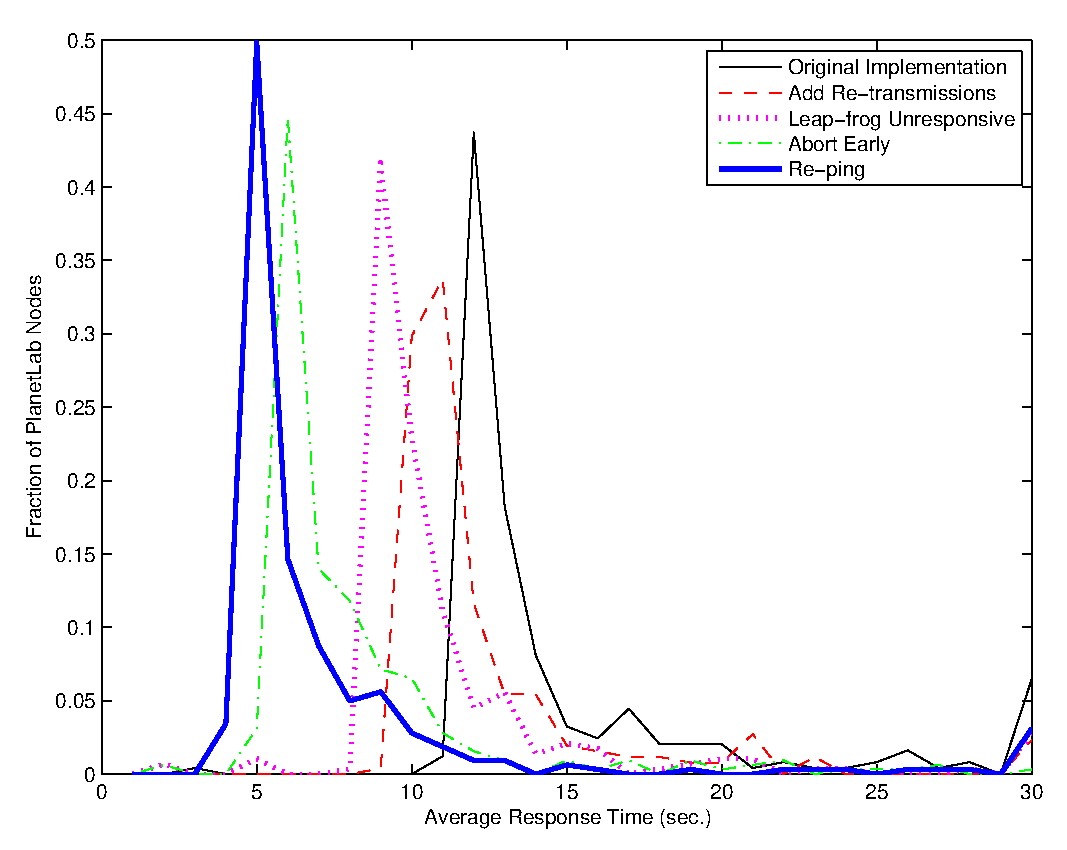
\includegraphics[width=\columnwidth]{apt_p2p_improvements-find_value.eps}
\caption{The distribution of average response times PlanetLab nodes
experience for \texttt{find\_value} queries. The original DHT
implementation results are shown, as well as the successive
improvements that we made to reduce the response time.}
\label{improvements}
\end{figure}

To test our changes during development, we ran the customized DHT
for several hours after each major change on 300 PlanetLab nodes
\cite{planetlab}. Though the nodes are not expected to be firewalled
or NATted, some can be quite overloaded and so consistently fail to
respond within a timeout period, similar to NATted peers. The
resulting distribution of the nodes' average response times is shown
in Figure~\ref{improvements}. Each improvement successfully reduced
the response time, for a total reduction of more than half. The
final distribution is also narrower, as the improvements make the
system more predictable. However, there are still a large number of
outliers with higher average response times, which are the
overloaded nodes on PlanetLab. This was confirmed by examining the
average time it took for a timeout to occur, which should be
constant as it is a configuration option, but can be much larger if
the node is too overloaded for the program to be able to check for a
timeout very often.

\subsection{Multiple Values}
\label{multiple_values}

The original design of Kademlia specified that each keywould have
only a single value associated with it. The RPC to find this value
was called \texttt{find\_value} and worked similarly to
\texttt{find\_node}, iteratively finding nodes with ID's closer to
the desired key. However, if a node had a value stored associated
with the searched for key, it would respond to the request with that
value instead of the list of nodes it knows about that are closer.

While this works well for single values, it can cause a problem when
there are multiple values. If the responding node is no longer one
of the closest to the key being searched for, then the values it is
returning will probably be the staler ones in the system, and it
will not have the latest stored values. However, the search for
closer nodes will stop here, as the queried node only returned the
values and not a list of nodes to recursively query. We could have
the request return both the values and the list of nodes, but that
would severely limit the size and number of the values that could be
returned.

Instead, we have broken up the original \texttt{find\_value}
operation into two parts. The new \texttt{find\_value} request
always returns a list of nodes that the node believes are closest to
the key, as well as a number indicating the number of values that
this node has for the key. Once a querying node has finished its
search for nodes and found the closest ones to the key, it can issue
\texttt{get\_value} requests to some nodes to actually retrieve the
values they have. This allows for much more control of when and how
many nodes to query for values. For example, a querying node could
abort the search once it has found enough values in some nodes, or
it could choose to only request values from the nodes that are
closest to the key being searched for.

\subsection{BitTorrent's Improvements}
\label{bittorrent_dht}

In the many years that some BitTorrent clients have been using a
Kademlia based DHT for tracker-less operation, the developers have
made many enhancements which we can take advantage of. One of the
most important is a security feature added to stop malicious nodes
from subscribing other nodes as downloaders. When a node issues a
request to another node to store its download info for that key, it
must include a \emph{token} returned by the storing node in a recent
\texttt{find\_node} request. The token is created by hashing the IP
address of the requesting peer with a temporary secret that expires
after several minutes. This prevents the requesting peer from faking
its IP address in the store request, since it must first receive a
response from a \texttt{find\_node} on that IP.

We also made some BitTorrent-inspired changes to the parameters of
the DHT originally specified by the authors of Kademlia. Since, as
we will show later, peers stay online in our system for much longer
periods of time, we reduced Kademlia's \emph{k} value from 20 to 8.
The value is supposed to be large enough such that any given
\emph{k} nodes are unlikely to fail within an hour of each other,
which is very unlikely in our system given the long uptimes of
nodes. We also increased the number of concurrent outstanding
requests allowed from 3 to 6 to speed up the recursive key finding
processes.

\subsection{Other Changes}
\label{other_changes}

We added one other new RPC request that nodes can make:
\texttt{join}. This request is only sent on first loading the DHT,
and is usually only sent to the bootstrap nodes that are listed for
the DHT. These bootstrap nodes will respond to the request with the
requesting peer's IP and port, so that the peer can determine what
its oustide IP address is and whether port translation is being
used. In the future, we hope to add functionality similar to STUN
\cite{STUN}, so that nodes can detect whether they are NATted and
take appropriate steps to circumvent it.

In addition, we have allowed peers to store values in the DHT, even
if the hash they are using is not the correct length. Most of the
keys used in the DHT are based on the SHA1 hash, and so they are 20
bytes in length. However, some files in the targetted Debian package
system are only hashed using the MD5 algorithm, and so the hashes
retrieved from the server are 16 bytes in length. The DHT will still
store values using these keys by padding the end of them with zeroes
to the proper length, as the loss of uniqueness from the 4 less
bytes is not an issue. Also, the DHT will happily store hashes that
are longer than 20 bytes, such as those from the 32 byte SHA256
algorithm, by truncating them to the correct length. Since the
requesting peer will have the full length of the hash, this will not
affect its attempt to verify the downloaded file.

%%%%%%%%%%%%%%%%%%%%%%%%%%%  Section  %%%%%%%%%%%%%%%%%%%%%%%%%%%%

\section{Performance Evaluation}
\label{analysis}

Our \texttt{apt-p2p} implementation supporting the Debian package
distribution system has been available to all Debian users since May
3rd, 2008 \cite{apt-p2p-debian}, and will also be available in the
next release of Ubuntu \cite{apt-p2p-ubuntu}. We have since created
a \emph{walker} that will navigate the DHT and find all the peers
currently connected to it. This allows us to analyze many aspects of
our implementation.

\subsection{Peer Lifetimes}
\label{peer_life}

\begin{figure}
\centering
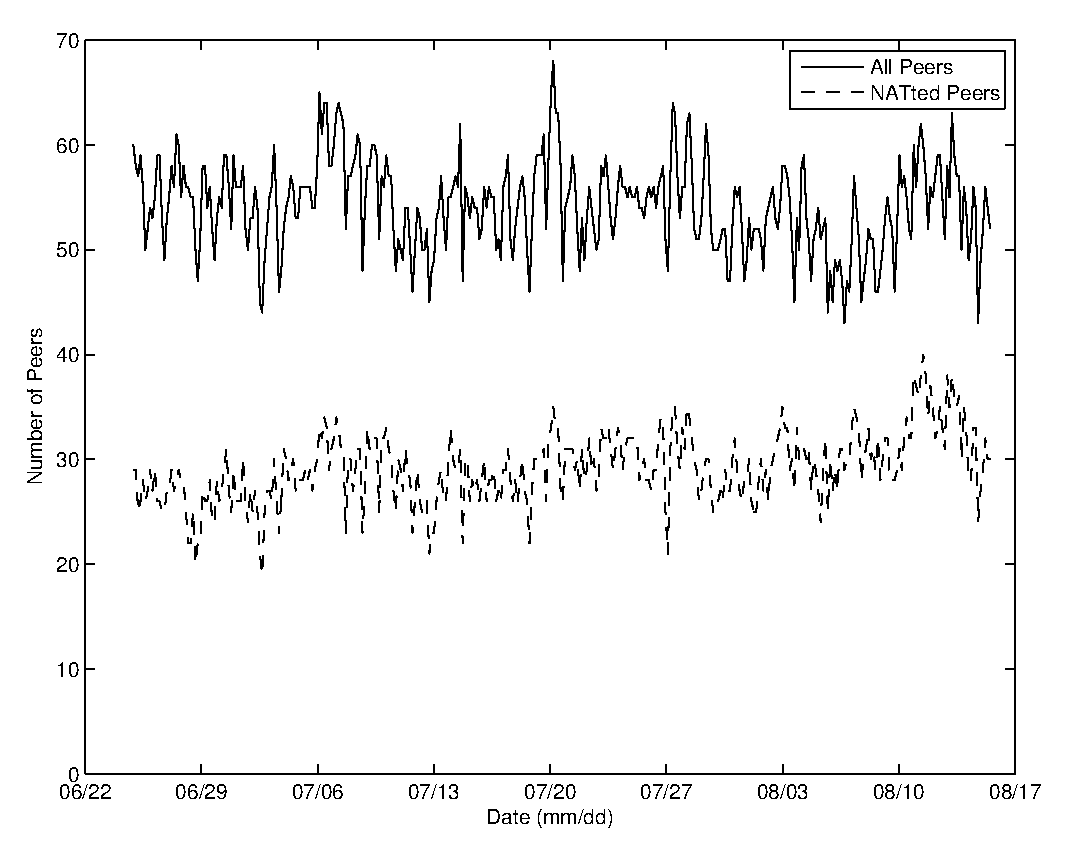
\includegraphics[width=\columnwidth]{AptP2PWalker-peers.eps}
\caption{The number of peers found in the system, and how many are
behind a firewall or NAT.}
\label{walker_peers}
\end{figure}

We first began analyzing the DHT on June 24th, and continue to this
day, giving us 2 months of data so far. Figure~\ref{walker_peers}
shows the number of peers we have seen in the DHT during this time.
The peer population is very steady, with just over 50 regular users
participating in the DHT at any time. We also note that we find 100
users who connect regularly (weekly), and we have found 186 unique
users in the 2 months of our analysis. We determined which users are
behind a firewall or NAT, which is one of the main problems of
implementing a peer-to-peer network. These peers will be
unresponsive to DHT requests from peers they have not contacted
recently, which will cause the peer to wait for a timeout to occur
(currently set at 9 seconds) before moving on. They will also be
unable to contribute any upload bandwidth to other peers, as all
requests for packages from them will also timeout. From
Figure~\ref{walker_peers}, we see that approximately half of all
peers suffered from this restriction.

\begin{figure}
\centering
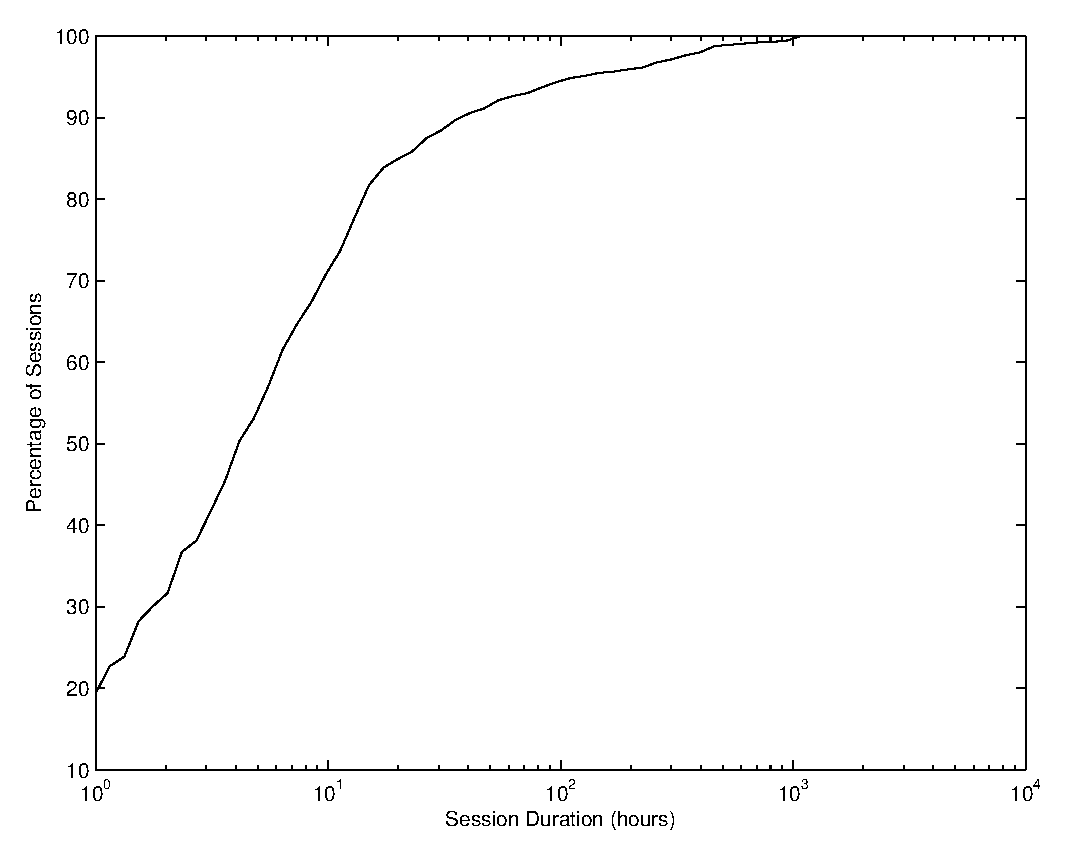
\includegraphics[width=\columnwidth]{AptP2PDuration-peers.eps}
\caption{The CDF of how long an average session will last.}
\label{duration_peers}
\end{figure}

Figure~\ref{duration_peers} shows the cumulative distribution of how
long a connection from a peer can be expected to last. Due to our
software being installed as a daemon that is started by default
every time their computer boots up, peers are expected to stay for a
long period in the system. 50\% of connections last longer than 5
hours, and 20\% last longer than 10 hours. These connections are
much longer than those reported by Saroiu et. al. \cite{saroiu2001}
for other P2P systems, which had 50\% of Napster and Gnutella
sessions lasting only 1 hour.

\begin{figure}
\centering
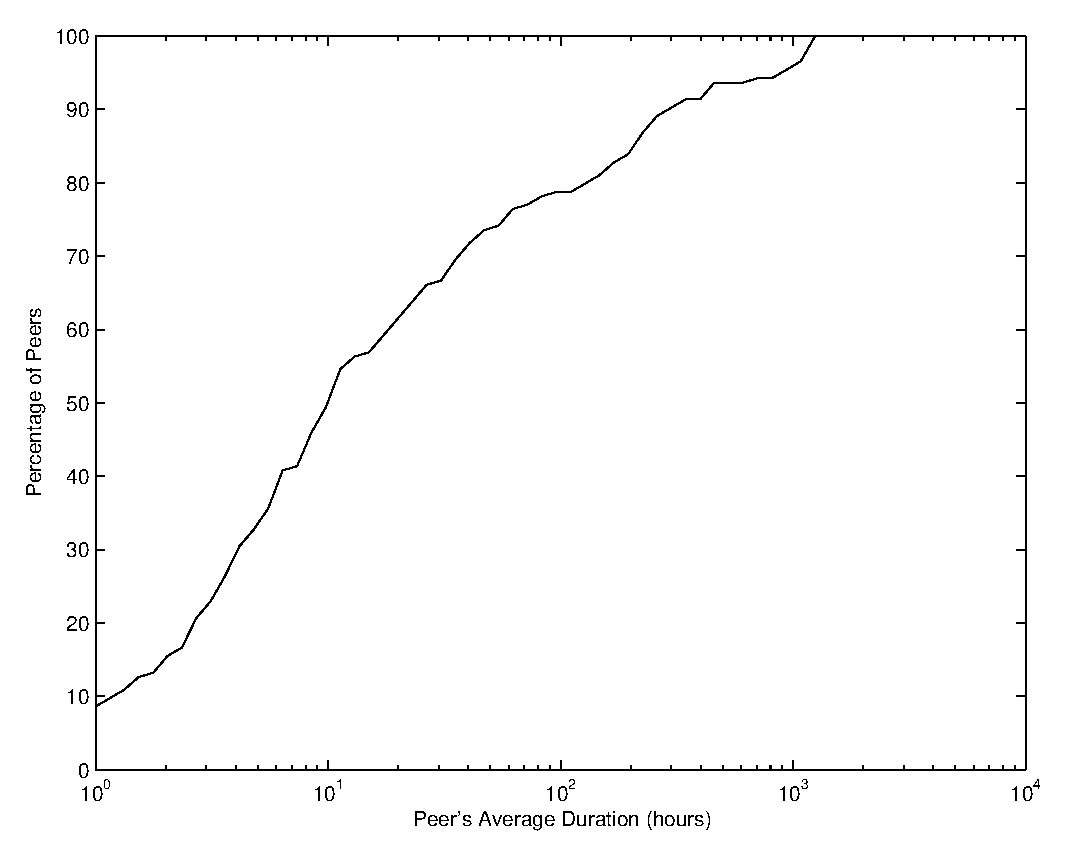
\includegraphics[width=\columnwidth]{AptP2PDuration-ind_peers.eps}
\caption{The CDF of the average time individual peers stay in the
system.}
\label{duration_ind_peers}
\end{figure}

We also examined the average time each individual peer spends in the
system. Figure~\ref{duration_peers} shows the cumulative
distribution of how long each individual peer remains in the system.
Here we see that 50\% of peers have average stays in the system
longer than 10 hours.

\begin{figure}
\centering
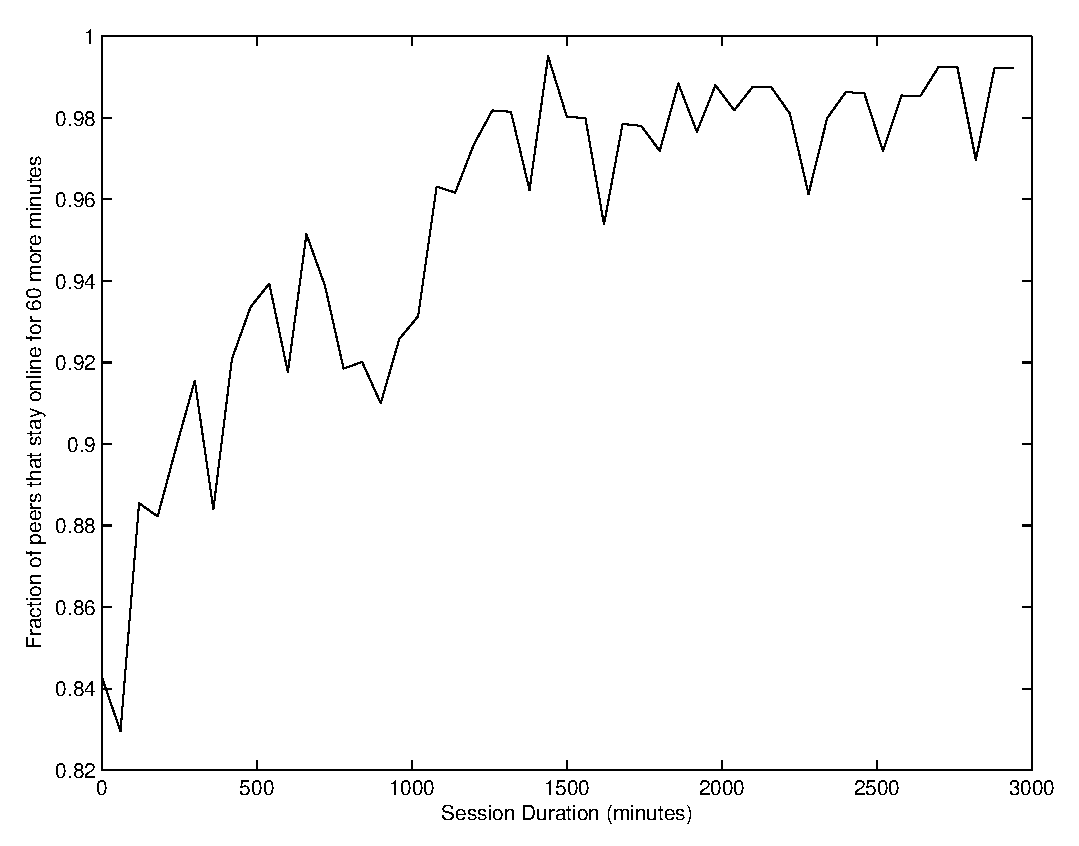
\includegraphics[width=\columnwidth]{AptP2PDuration-online_1.eps}
\caption{The fraction of peers that, given their current duration in
the system, will stay online for another hour.}
\label{duration_online_1}
\end{figure}

Since our DHT is based on Kademlia, which was designed based on the
probability that a node will remain up another hour, we also
analyzed our system for this parameter.
Figure~\ref{duration_online_1} shows the fraction of peers will
remain online for another hour, as a function of how long they have
been online so far. Maymounkov and Mazieres found that the longer a
node has been online, the higher the probability that it will stay
online \cite{kademlia}. Our results also show this behavior. In
addition, similar to the Gnutella peers, over 90\% of our peers that
have been online for 10 hours, will remain online for another hour.
Our results also show that, for our system, over 80\% of all peers
will remain online another hour, compared with around 50\% for
Gnutella.

\begin{figure}
\centering
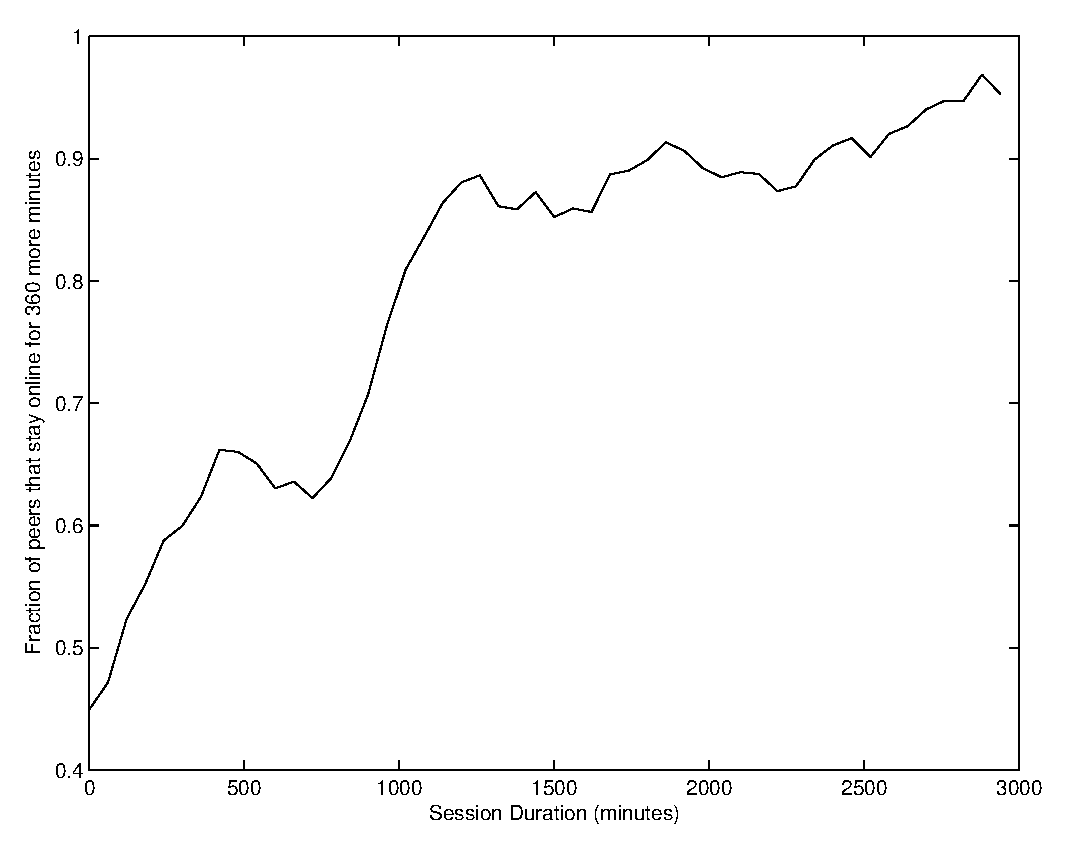
\includegraphics[width=\columnwidth]{AptP2PDuration-online_6.eps}
\caption{The fraction of peers that, given their current duration in
the system, will stay online for another 6 hours.}
\label{duration_online_6}
\end{figure}

Since our peers are much longer-lived than other P2P systems, we
also looked at the fraction of peers that stay online for another 6
hours. Figure~\ref{duration_online_6} shows that over 60\% of peers
that are online for 10 hours will stay online for another 6.
However, we see an interesting decrease in this fraction between 8
and 12 hours, which can also be seen in
Figure~\ref{duration_online_1}. We believe this to be due to desktop
users, who regularly turn off their computers at night.

\subsection{Peer Statistics}
\label{peer_stats}

On July 31st we enhanced our walker to retrieve additional
information from each contacted peer. The peers are configured, by
default, to publish some statistics on how much they are downloading
and uploading, and their measured response times for DHT queries.
Our walker can extract this information if the peer is not
firewalled or NATted, it has not disabled this functionality, and if
it uses the same port for both its DHT (UDP) requests and download
(TCP) requests (which is also a configuration parameter).

\begin{figure}
\centering
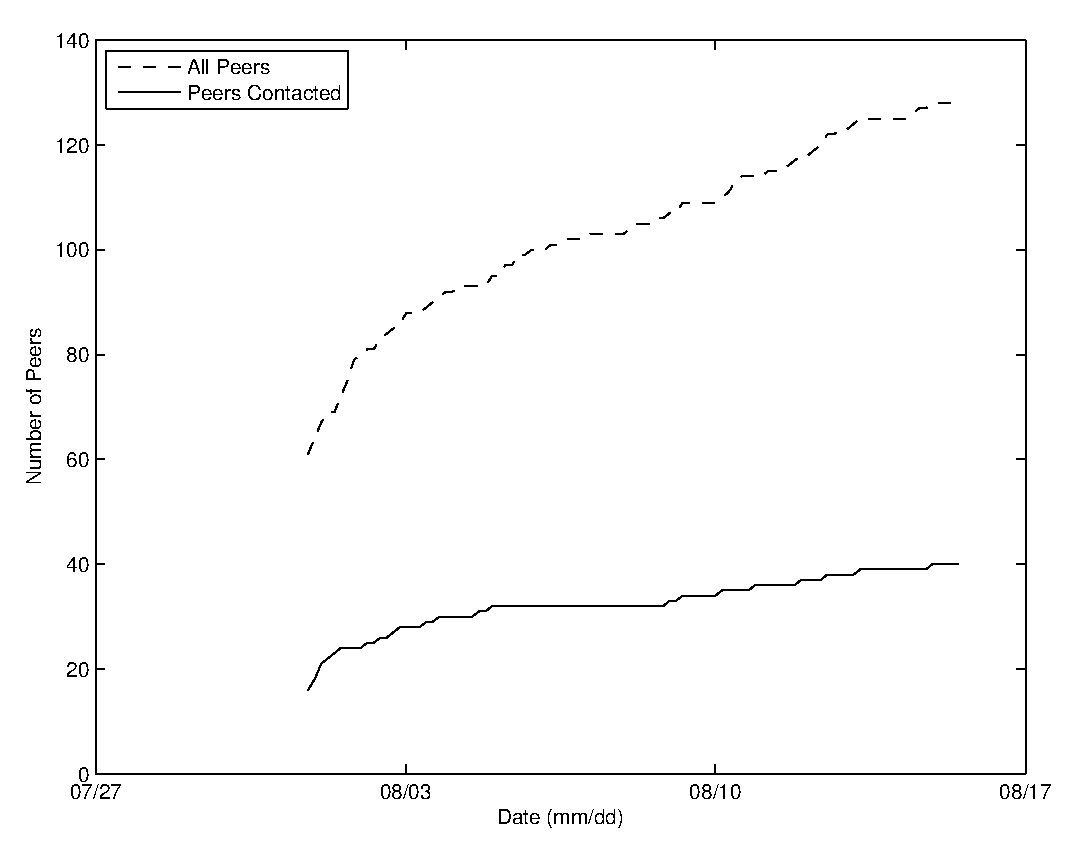
\includegraphics[width=\columnwidth]{AptP2PDownloaded-peers.eps}
\caption{The number of peers that were contacted to determine their
bandwidth, and the total number of peers in the system.}
\label{down_peers}
\end{figure}

Figure~\ref{down_peers} shows the total number of peers we have been
able to contact since starting to gather this additional
information, as well as how many total peers were found. We were
only able to contact 30\% of all the peers that connected to the
system during this time.

\begin{figure}
\centering
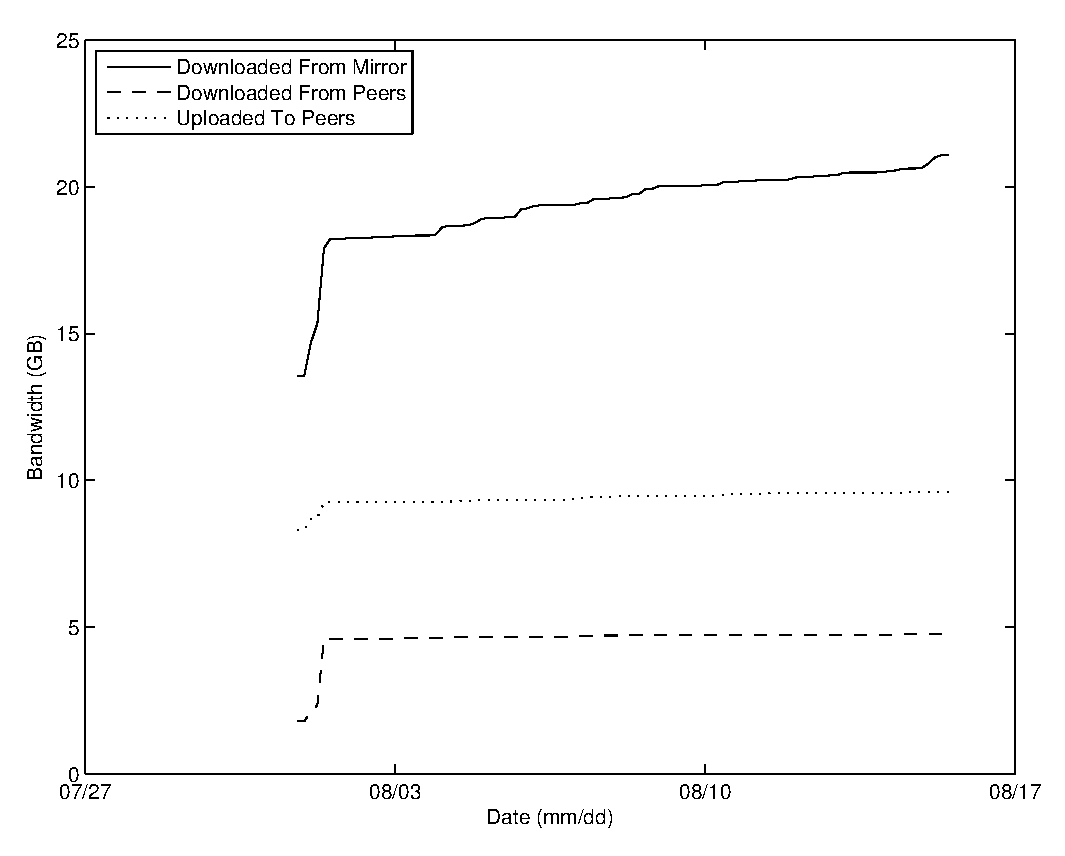
\includegraphics[width=\columnwidth]{AptP2PDownloaded-bw.eps}
\caption{The bandwidth of data that the contacted peers have
downloaded and uploaded.}
\label{down_bw}
\end{figure}

Figure~\ref{down_bw} shows the amount of data the peers we were able
to contact have downloaded. Peers measure their downloads from other
peers and mirrors separately, so we are able to get an idea of how
much savings our system is generating for the mirrors. We see that
the peers are downloading approximately 20\% of their package data
from other peers, which is saving the mirrors from supplying that
bandwidth. The actual numbers are only a lower bound, since we have
only contacted 30\% of the peers in the system, but we can estimate
that \texttt{apt-p2p} has already saved the mirrors 15 GB of
bandwidth, or 1 GB per day.

We also collected the statistics on the measured response time peers
were experiencing when sending requests to the DHT. We found that
the recursive \texttt{find\_value} query, which is necessary before
a download can occur, is taking 17 seconds on average. This
indicates that, on average, requests are experiencing almost 2
stalls while waiting for the 9 second timeouts to occur on
unresponsive peers. This is longer than our target of 10 seconds,
although it will only lead to a slight average delay in downloading
of 1.7 seconds when the default 10 concurrent downloads are
occurring.This increased response time is due to the number of peers
that were behind firewalls or NATs, which was much higher than we
anticipated. We do have plans to improve this through better
informing of users of their NATted status, the use of STUN
\cite{STUN} to circumvent the NATs, and by better exclusion of
NATted peers from the DHT (which will not prevent them from using
the system).

We were also concerned that the constant DHT requests and responses,
even while not downloading, would overwhelm some peers' network
connections. However, we found that peers are using 200 to 300 bytes
per second of bandwidth in servicing the DHT. These numbers are
small enough to not affect any other network services the peer would
be running.


%%%%%%%%%%%%%%%%%%%%%%%%%%%  Section  %%%%%%%%%%%%%%%%%%%%%%%%%%%%

\section{Related Work}
\label{related}

There have also been preliminary attempts to implement peer-to-peer distributors for
software packages. apt-torrent \cite{apttorrent} creates torrents
for some of the larger packages available, but it ignores the
smaller packages, which are often the most popular. DebTorrent
\cite{debtorrent} makes widespread modifications to a traditional
BitTorrent client, to try and fix the drawbacks mentioned in
Section~\ref{bittorrent}. However, these changes also require some
modifications to the distribution system to support it. Our system
considers all the files available to users to download, and makes
use of the existing infrastructure unmodified.

Others have also used DHTs to support this type of functionality.
Kenosis \cite{kenosis} is a P2P Remote Procedure Call
client also based on the Kademlia DHT, but it is meant as a P2P
primitive system on which other tools can be built, and so it has no
file sharing functionality at all. Many have used a DHT as a drop-in
replacement for the tracker in a BitTorrent system
\cite{bittorrent-dht, azureus-dht}, but such systems only use the
DHT to find peers for the same torrent, so the file sharing uses
traditional BitTorrent and so is not ideal for the reasons listed
in Section~\ref{bittorrent}.

% \cite{deltacast}

There are a number of works dedicated to developing a collaborative
content distribution network (CDN) using peer-to-peer techniques.
Freedman et. al. developed Coral \cite{coral} using a distrbitued
\emph{sloppy} hash table to speed request times. Pierre and van
Steen developed Globule \cite{globule} which uses typical DNS and
HTTP redirection techniques to serve requests from a network of
replica servers, which in turn draw their content from the original
location (or a backup). Shah et. al. \cite{shah08} analyze an
existing software delivery system and use the results to design a
peer-to-peer content distribution network that makes use of
volunteer servers to help with the load. None of these systems meets
our goal of an even distribution of load amongst the users of the
system. Not all users of the systems become peers, and so are not
able to contribute back to the system after downloading. The
volunteers that do contribute as servers are required to contribute
larger amounts of bandwidth, both for uploading to others, and in
downloading content they are not in need of in order to share them
with other users. Our system treats all users equally, requiring all
to become peers in the system, sharing the uploading load equally
amongst all, but doesn't require any user to download files they
would not otherwise need.

The most similar works to ours are by Shah et. al. \cite{shah08} and
Shark by Annapureddy et. al. \cite{shark}.
Shah's system, in addition to the drawbacks mentioned previously,
is not focused on the interactivity of downloads, as
half of all requests were required ``to wait between 8 and 15
minutes.'' In contrast, lookups in our system take only seconds to
complete, and all requests can be completed in under a minute.
Shark makes use of Coral's distributed sloppy hash table to speed
the lookup time, but their system is more suited to its intended use
as a distributed file server. It doesn't make use of authoritative
copies of the original files, allowing instead any users in the
system to update files and propagate those changes to others. Our
system is well-tailored to the application of disseminating the
unchanging software packages from the authoritative sources to all
users unchanged.


%%%%%%%%%%%%%%%%%%%%%%%%%%%  Section  %%%%%%%%%%%%%%%%%%%%%%%%%%%%

\section{Conclusion and Future Work}
\label{conclusions}

We have designed a generally applicable peer-to-peer content
distribution model to be used by many of the free software
distributors operating today. It makes use of already existing
features of most package management systems to create a
peer-to-peer distribution that should substantially reduce the costs
of hosting the software packages.

We have also implemented our design in freely available software to
be used in conjuction with Debian-based distribution of Linux
software packages. It is currently in use by some users of the
Debian project's distribution, and so serves as an example of the
possibilities that exist.

We feel that our P2P software package distribution model is
well-suited to be used by many free software distributors. We hope
to convince them to adopt such a model in their distribution, or we
may port our existing system to some of the other groups for them to
try.

One aspect missing from our model is the removal of old packages
from the cache. Since our implementation is still relatively young,
we have not had to deal with the problems of a growing cache of
obsolete packages consuming all of a user's hard drive. We plan to
implement some form of least recently used (LRU) cache removal
technique, in which packages that are no longer available on the
server, no longer requested by peers, or simply are the oldest in
the cache, will be removed.

The most significant area of improvement still needed in our sample
implementation is to further speed up some of the slower recursive
DHT requests. We hope to accomplish this by further tuning the
parameters of our current system, better exclusion of NATted peers
from the routing tables, and through the use of STUN \cite{STUN} to
circumvent the NATs of the 50\% of the peers that have not
configured port forwarding.

\bibliographystyle{IEEEtran}
\bibliography{./IEEEabrv,./all}

\end{document}
